\subsection{Расчет скоростей нейтронного захвата в программе TALYS}
В настоящей работе для исследования чувствительности модели $r$-процесса к выбору теоретических значений масс нейтроноизбыточных ядер мы рассчитали скорости реакции $(n,\gamma)$ $r$-процесса с помощью программы TALYS~\cite{koning2019}, используя три различные массовые таблицы: FRDM2012, HFB-24 и LMR2021. В настоящем разделе обсуждаются некоторые практические детали проведенных расчетов и анализируются их результаты.

\subsubsection{Массы ядер как параметры расчета}
Программа TALYS~\cite{koning2019}, которую мы использовали для расчета сечений и скоростей реакции $(n,\gamma)$, позволяет задавать различные параметры статистической модели, в том числе теоретические массы ядер. Мы использовали микро-коллективную модель FRDM2012~\cite{moller2016} и микроскопическую модель HFB-24~\cite{goriely2013}, внесенные в состав пакета TALYS его разработчиками, а также феноменологический метод LMR2021, предсказания которого были переведены нами в формат TALYS. 

Помимо таблиц теоретических масс ядер, в TALYS внесена таблица экспериментальных масс, построенная на основе базы данных AME2003~\cite{wapstra2003}. В наших расчетах при наличии экспериментальных масс предпочтение отдавалось им. Наконец, если при расчете TALYS требуются значения масс, отсутствующие и в экспериментальной, и в теоретической таблице, то программа использует аналитическую формулу Дуфло-Цукера~\cite{duflo1995}.

\subsubsection{Модификация исходного кода TALYS}
В исходный код программы TALYS нами было внесено изменение, делающее сетку температур, по которой производится расчет астрофизических скоростей, равномерной и более густой. Эта правка никак не влияет на работу статистической модели ядерных реакций, лишь делает выходные данные более подробными ценой некоторого увеличения времени расчета. Все расчеты TALYS, использовавшиеся в настоящей работе, получены на этой измененной версии программы.  

\subsubsection{Результаты расчета сечений реакции $(n,\gamma)$ с помощью TALYS}

\begin{figure}
  \centering
  \begin{subfigure}{0.48\textwidth}
    \centering
    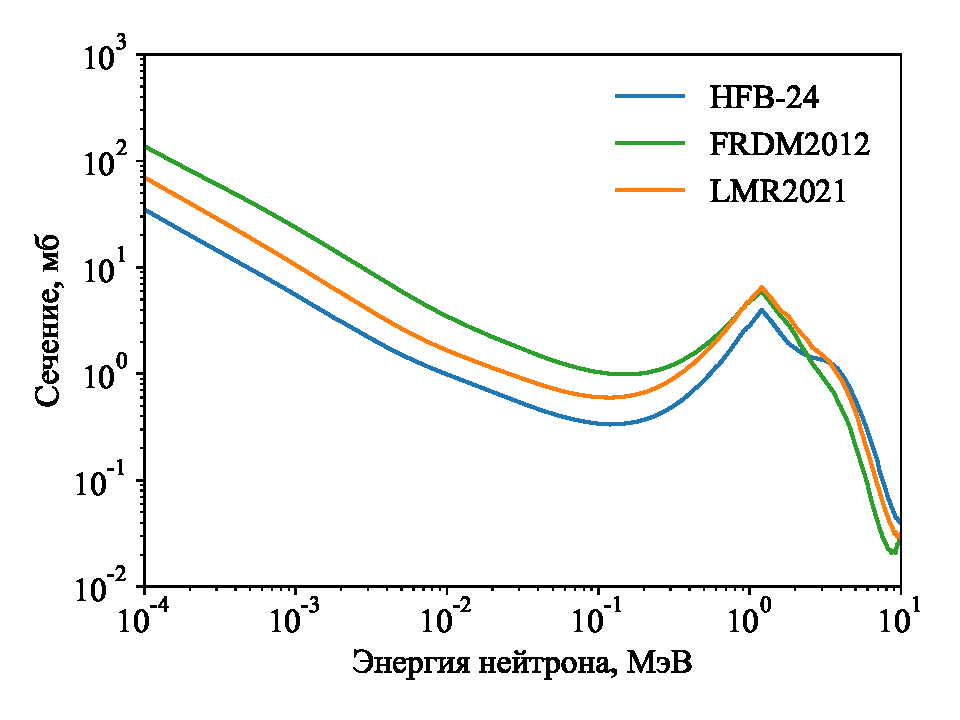
\includegraphics[width=\textwidth]{../pics/cs_in141.pdf}
    \caption{${}^{141}$In}
  \end{subfigure}
  \hfill
  \begin{subfigure}{0.48\textwidth}
    \centering
    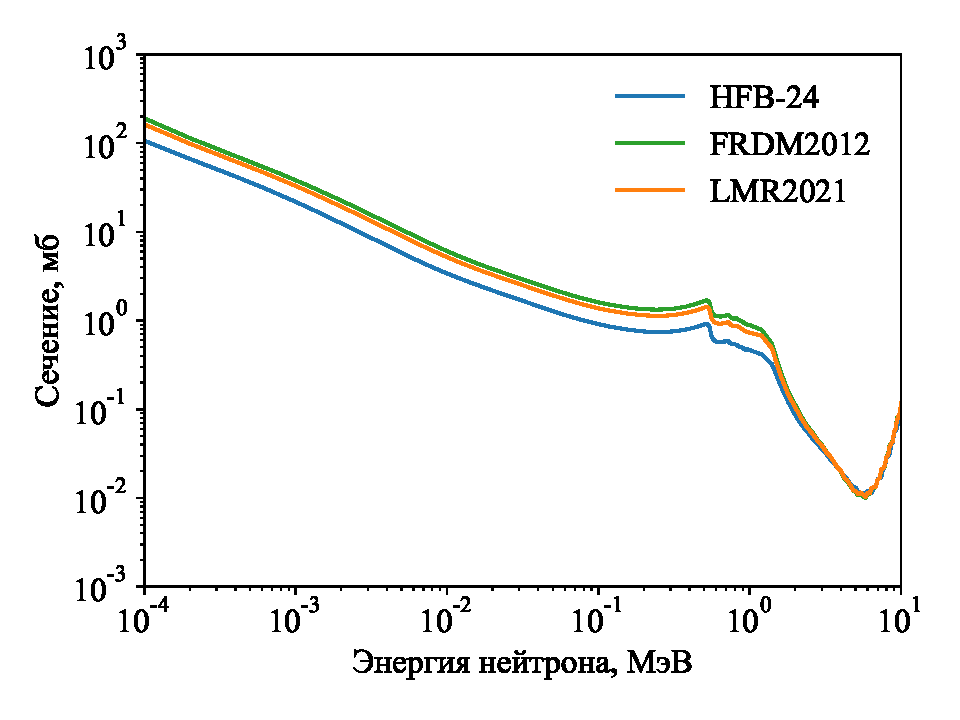
\includegraphics[width=\textwidth]{../pics/cs_in142.pdf}
    \caption{${}^{142}$In}
  \end{subfigure}
  \\
  \begin{subfigure}{0.48\textwidth}
    \centering
    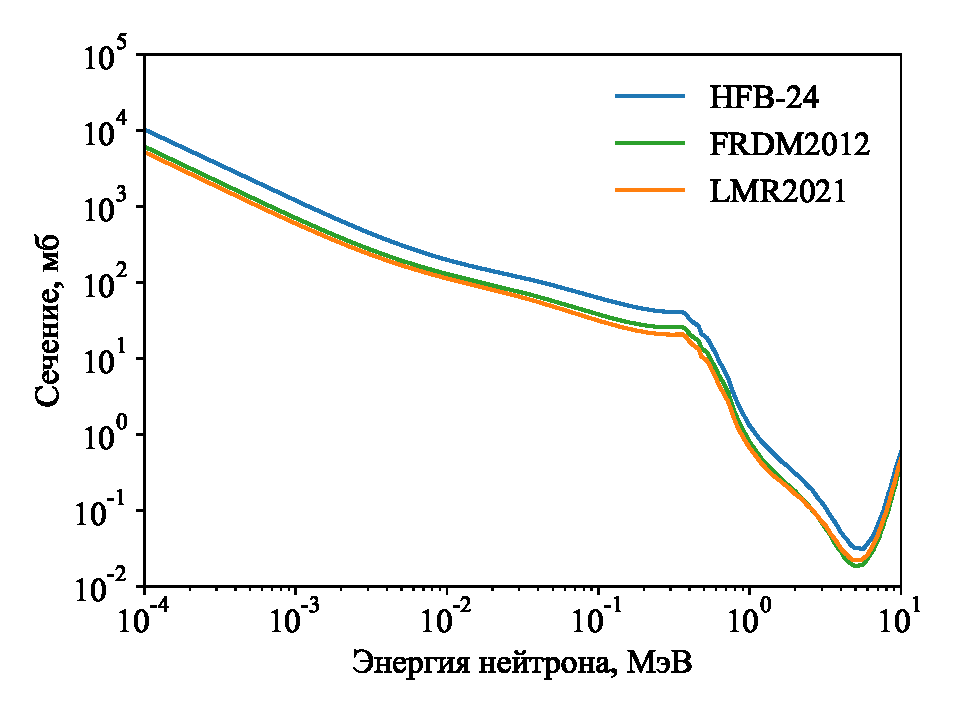
\includegraphics[width=\textwidth]{../pics/cs_tb186.pdf}
    \caption{${}^{186}$Tb}
  \end{subfigure}
  \hfil
  \begin{subfigure}{0.48\textwidth}
    \centering
    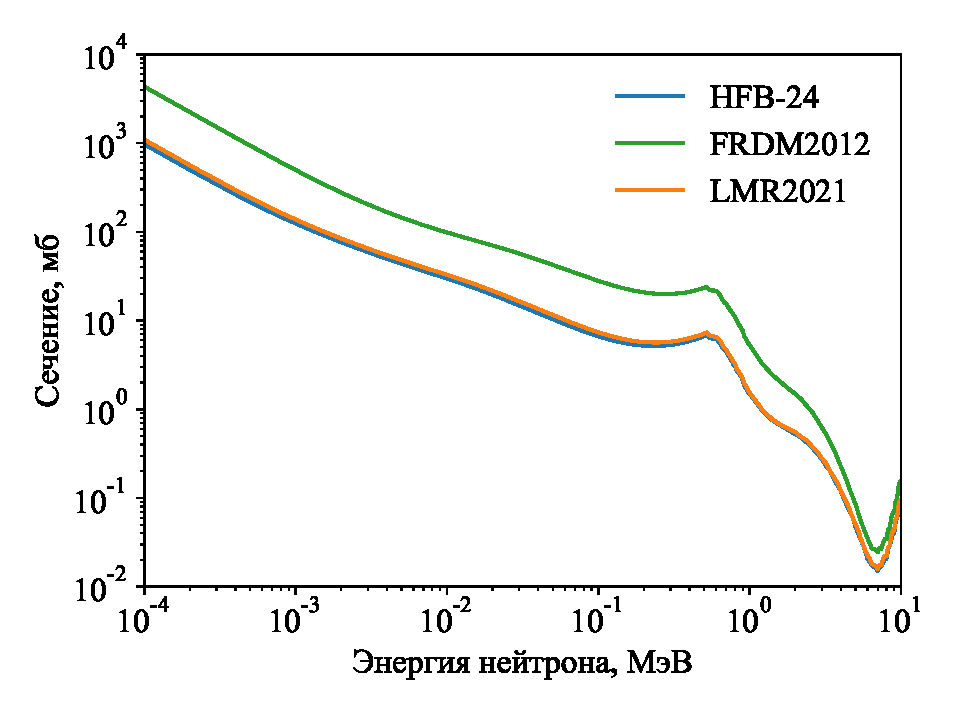
\includegraphics[width=\textwidth]{../pics/cs_tb187.pdf}
    \caption{${}^{187}$Tb}
  \end{subfigure}
  \\
  \begin{subfigure}{0.48\textwidth}
    \centering
    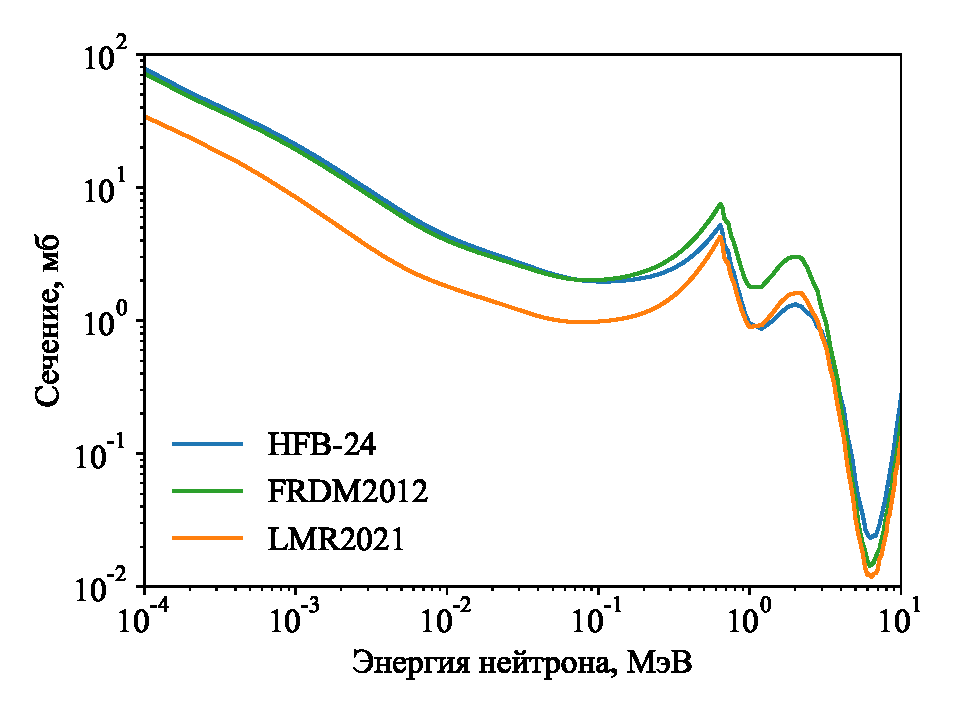
\includegraphics[width=\textwidth]{../pics/cs_pb236.pdf}
    \caption{${}^{236}$Pb}
    \label{fig:ng_cs:236pb}
  \end{subfigure}
  \hfil
  \begin{subfigure}{0.48\textwidth}
    \centering
    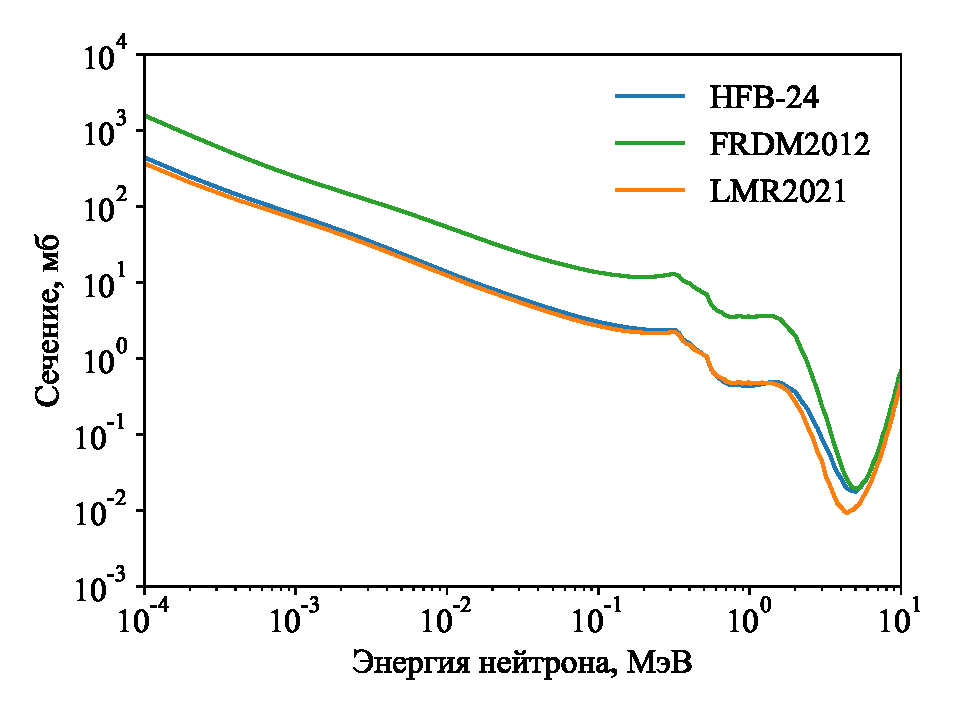
\includegraphics[width=\textwidth]{../pics/cs_pb237.pdf}
    \caption{${}^{237}$Pb}
    \label{fig:ng_cs:237pb}
  \end{subfigure}
  \caption{Сечения реакции $(n,\gamma)$ на некоторых нейтроноизбыточных изотопах индия, тербия и свинца, полученные с помощью программы TALYS с использованием различных массовых моделей.}
  \label{fig:ng_cs}
\end{figure}

В режиме расчета астрофизических скоростей TALYS вычисляет сечения реакции и интегрирует их в соответствии с формулой~(\ref{eq:rate}). Прежде чем искать скорости реакций, мы запустили TALYS в режиме расчета сечений для ряда реакций нейтронного захвата, используя значения масс FRDM2012, HFB-24 и LMR2021, чтобы проанализировать влияние массовой модели на величины сечений. Результаты представлены на рис.~\ref{fig:ng_cs}. Как видно, наибольшие различия в сечениях, полученных с использованием разных массовых моделей, относятся к низкоэнергетической области, в то время как при энергиях $5-10$~МэВ графики оказываются очень схожи и могут даже, как в случае с реакций ${}^{142}\text{In}(n,\gamma){}^{143}\text{In}$, практически сливаться. При этом как раз энергии частиц до $0.5$~МэВ наиболее интересны с точки зрения астрофизики. Таким образом можно ожидать существенного влияния выбора массовой ядерной модели на результаты моделирования $r$-процесса.

Видно, что в ряде случаев сечения, полученные при помощи массовой модели FRDM2012, превышают остальные сечения, однако это не всегда так: например, в реакции  ${}^{186}\text{Tb}(n,\gamma){}^{187}\text{Tb}$ сечение для массовой модели HFB-24. Заметно также, что для ядер с нечетным числом нейтронов вариация массовой модели приводит к большим расхождениям в сечениях $(n,\gamma)$, чем для соседних изотопов с четным числом нейтронов. Например, на рис.~\ref{fig:ng_cs:236pb} сечение $(n,\gamma)$ на четно-четном ядре ${}^{236}$Pb, полученное при помощи модели LMR2021, заметно отличается от результатов остальных массовых моделей, однако это различие не превышает отклонение спектра FRDM2012 от спектров прочих моделей для нейтронного захвата на изотопе ${}^{237}$Pb с одним неспаренным нейтроном (см. рис.~\ref{fig:ng_cs:237pb}).

Любопытно, как разные массовые модели показывают стремление к некому единому пределу в тех или иных областях энергий. Уже отмечалось, что при энергиях выше 5~МэВ зависимости сечений $(n,\gamma)$ для многих ядер сходятся. Для изотопа ${}^{141}$In наблюдается сближение сечений FRDM2012 и LMR2021 вблизи пика некого порогового эффекта при энергии 1~МэВ. Для изотопа ${}^{236}$Pb сечения HFB-24 и FRDM2012 очень близки в области низких энергий, однако при энергиях выше $0.1$~МэВ сечение HFB-24 становится ближе к результатам модели LMR2021. Напротив, у изотопа ${}^{237}$Pb сначала наблюдается близость сечений HFB-24 и LMR2021, но при энергии около 2~МэВ они расходятся, и график HFB-24 устремляется к графику сечений, полученному при помощи модели FRDM2012. Все это указывает на сложную связь сечений и ядерных масс.

\subsubsection{Результаты расчета скорости реакции $(n,\gamma)$ с помощью TALYS}

\begin{figure}
  \centering
  \begin{subfigure}{0.48\textwidth}
    \centering
    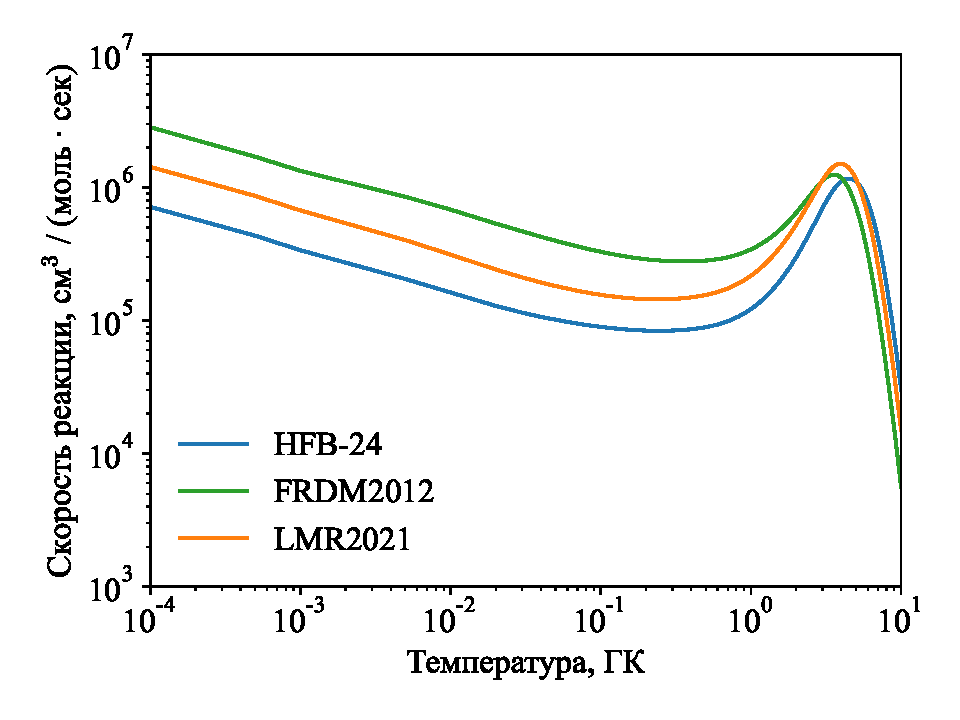
\includegraphics[width=\textwidth]{../pics/rate_in141.pdf}
    \caption{${}^{141}$In}
    \label{fig:ng_rate:141in}
  \end{subfigure}
  \hfill
  \begin{subfigure}{0.48\textwidth}
    \centering
    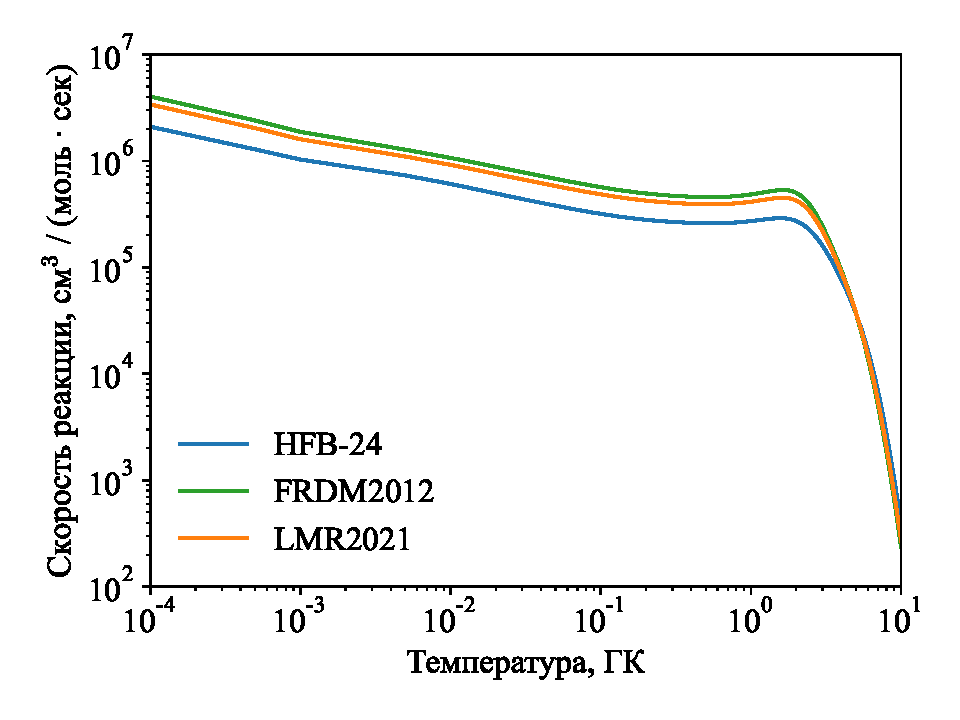
\includegraphics[width=\textwidth]{../pics/rate_in142.pdf}
    \caption{${}^{142}$In}
  \end{subfigure}
  \\
  \begin{subfigure}{0.48\textwidth}
    \centering
    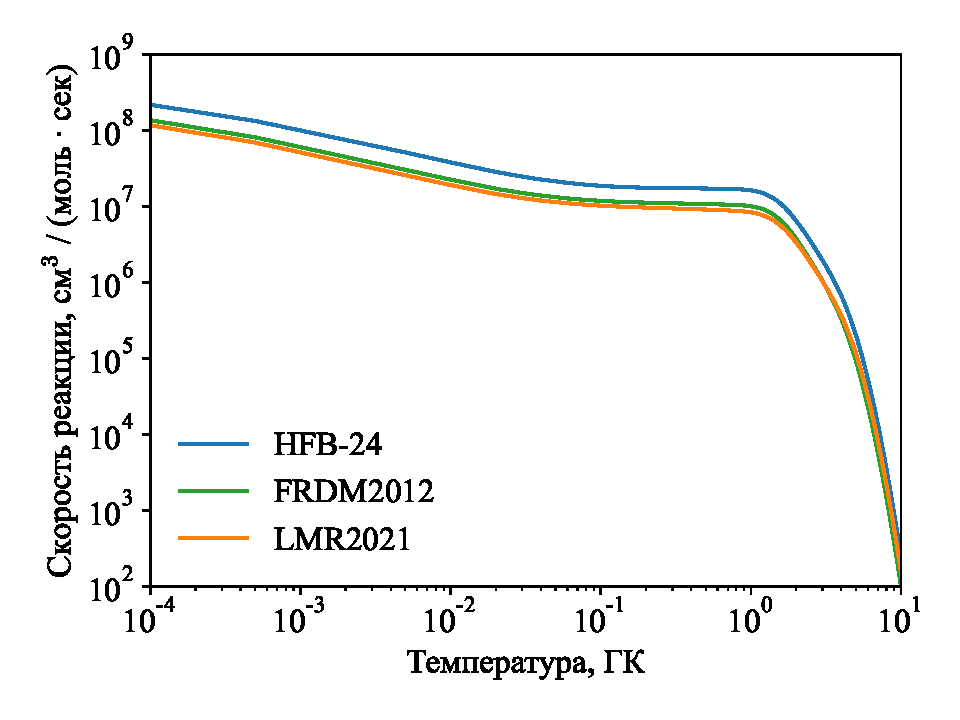
\includegraphics[width=\textwidth]{../pics/rate_tb186.pdf}
    \caption{${}^{186}$Tb}
  \end{subfigure}
  \hfil
  \begin{subfigure}{0.48\textwidth}
    \centering
    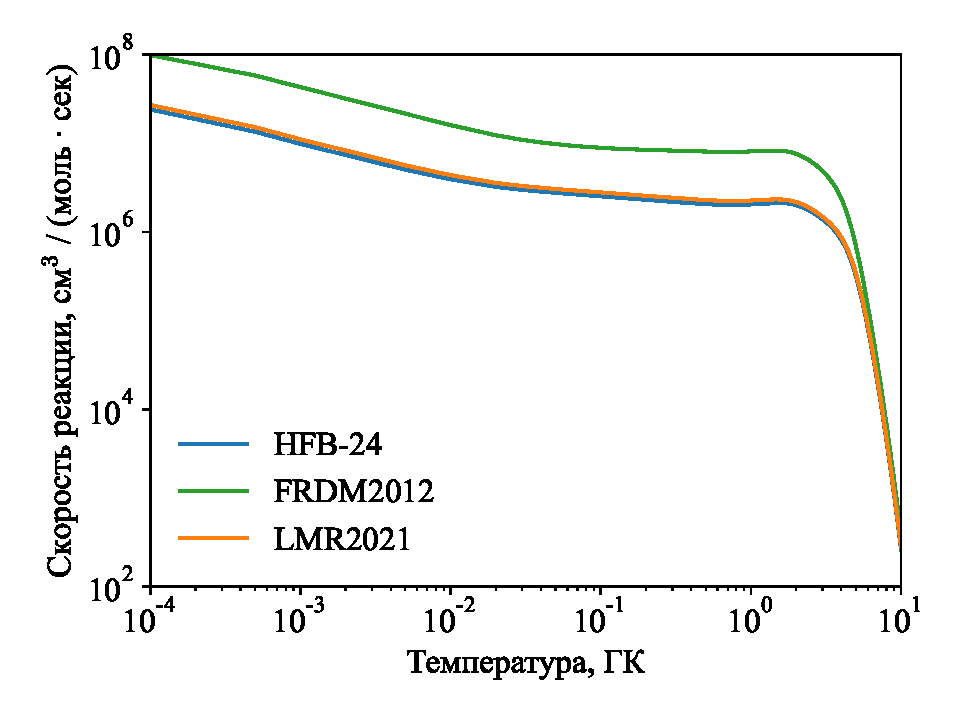
\includegraphics[width=\textwidth]{../pics/rate_tb187.pdf}
    \caption{${}^{187}$Tb}
  \end{subfigure}
  \\
  \begin{subfigure}{0.48\textwidth}
    \centering
    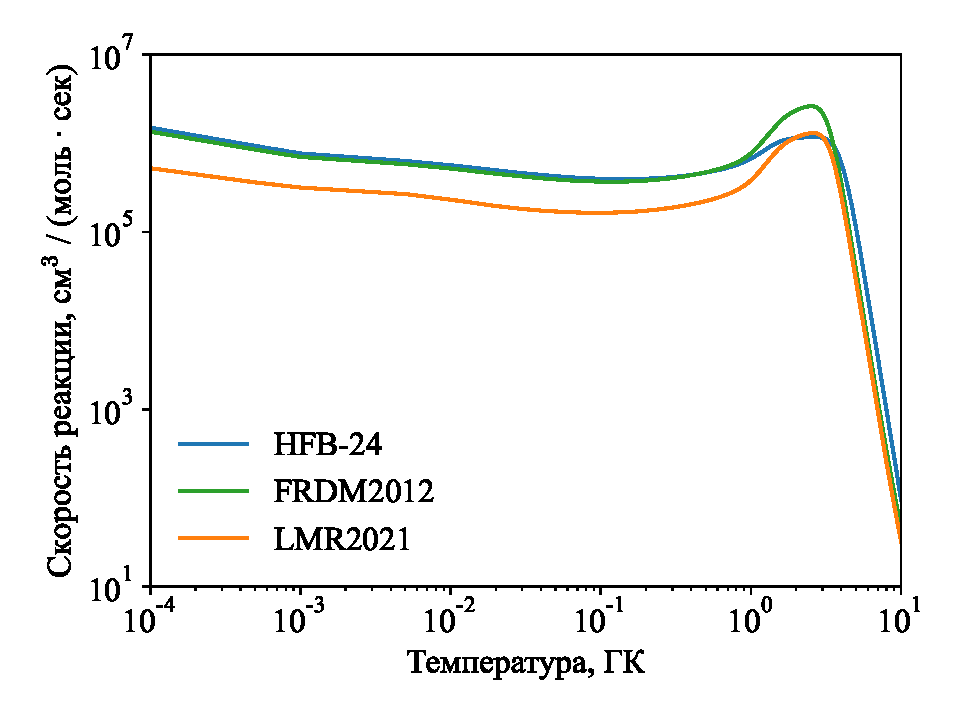
\includegraphics[width=\textwidth]{../pics/rate_pb236.pdf}
    \caption{${}^{236}$Pb}
    \label{fig:ng_rate:236pb}
  \end{subfigure}
  \hfil
  \begin{subfigure}{0.48\textwidth}
    \centering
    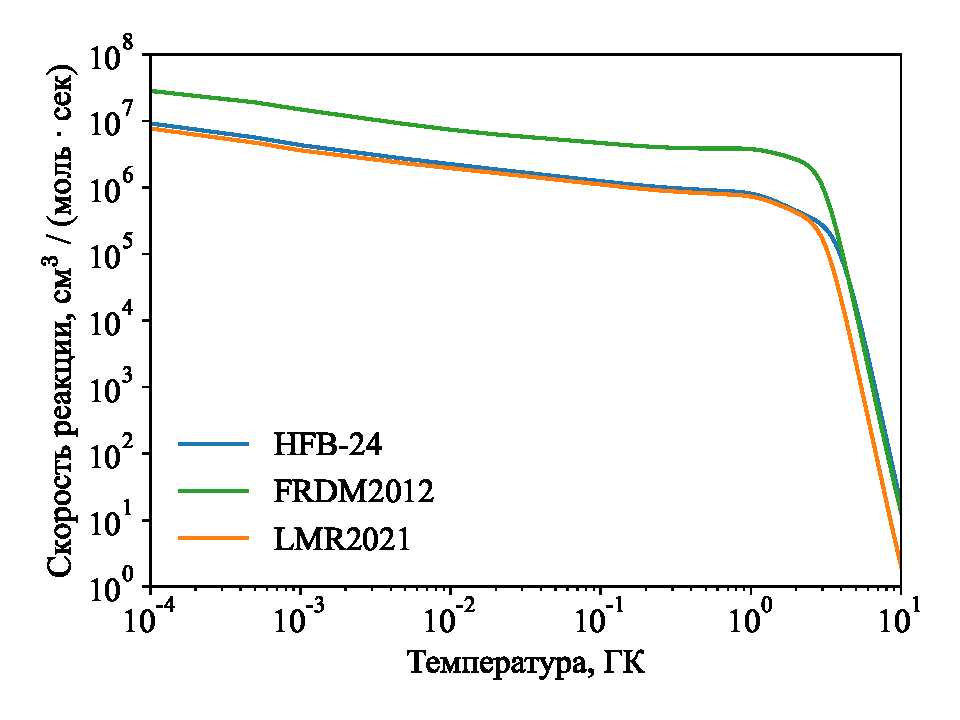
\includegraphics[width=\textwidth]{../pics/rate_pb237.pdf}
    \caption{${}^{237}$Pb}
    \label{fig:ng_rate:237pb}
  \end{subfigure}
  \caption{Скорости реакции $(n,\gamma)$ на некоторых нейтроноизбыточных изотопах индия, тербия и свинца, полученные с помощью программы TALYS с использованием различных массовых моделей.}
  \label{fig:ng_rate}
\end{figure}

При помощи программы TALYS нами были выполнены расчеты скорости реакции $(n,\gamma)$ на каждом изотопе, содержащемся в массовых таблицах FRDM2012, HFB-24 и LMR2021, с использованием содержащихся в них теоретических значений масс. Результаты расчетов для некоторых нейтроноизбыточных ядер-мишеней представлены на рис.~\ref{fig:ng_rate}. 

Поскольку скорость реакции получают путем свертки сечения реакции с распределением взаимодействующих частиц по энергии, представленные результаты соотносятся с графиками сечений на рис.~\ref{fig:ng_cs}. Точно также в области высоких температур (т.е. высоких средних энергий частиц) присутствует сближение скоростей, полученных с использованием разных массовых моделей. С другой стороны, как и в случае с сечениями, чувствительность расчета скоростей к выбору массовой модели для ядер с нечетным числом нейтронов оказывается выше, чем для соседних изотопов с четным числом нейтронов. Особенно хорошо это видно по графику скорости реакции ${}^{141}\text{In}(n,\gamma){}^{142}\text{In}$ на рис.~\ref{fig:ng_rate:141in} с различиями в области низких температур почти на порядок. Для изотопов свинца на рис.~\ref{fig:ng_rate:236pb} и \ref{fig:ng_rate:237pb}, как и в случае с сечениями, скорость HFB-24 при низких температурах тяготеет к результатам FRDM2012 и LMR2021, соответственно, но в области высоких температур устремляется к результатам другой модели.

\subsubsection{Нейтронный захват за границей существования ядер}
Во всех рассмотренных нами массовых таблицах присутствуют изотопы, находящиеся за областью существования ядер, то есть имеющие отрицательные энергии отделения протона $B_p$ или нейтрона $B_n$:
\begin{equation}\begin{aligned}\label{eq:driplines}
B_p(A,Z) &= E_{\text{св}}(A,Z) - E_{\text{св}}(A-1,Z-1),\\
B_n(A,Z) &= E_{\text{св}}(A,Z) - E_{\text{св}}(A-1,Z),
\end{aligned}\end{equation}
где $E_{\text{св}}$ --- энергия связи ядра, зависящая от выбора массовой модели. При отрицательных значениях $B_p$ или $B_n$ ядро фактически не существует. 

Мы провели расчеты скоростей нейтронного захвата в том числе и на этих несуществующих ядрах, чтобы убедиться, что их учет при моделировании $r$-процесса не будет приводить к некорректным результатам. На рис.~\ref{fig:rates_vs_A} представлены зависимости теоретических скоростей реакции $(n,\gamma)$ при $T = 2$~ГК на нейтроноизбыточных изотопах тербия, а также энергии отделения нейтрона $B_n$ для тех же ядер, рассчитанные по данным рассматриваемых нами массовых моделей. Как видно, начиная с массового числа $192$ для некоторых, в первую очередь нечетно-нечетных изотопов $B_n$ резко падает, доходя до отрицательных значений. При этом начинаются сильные колебания скорости $(n,\gamma)$: если конечное ядро имеет отрицательную $B_n$, то и скорость реакции снижается на порядки. 

Таким образом включение реакций $(n,\gamma)$ с образованием несвязанных нейтроноизбыточных ядер в симуляцию $r$-процесса не должно существенно повлиять на результаты моделирования. С другой стороны, учет таких реакций оставляет модели $r$-процесса возможность для некоторой инерции за границы существования. Путь $r$-процесса будет не просто упираться в линию отделения нейтрона из-за отсутствия возможности продвинуться дальше, а естественным образом замедляться.  

\begin{figure}
  \centering
  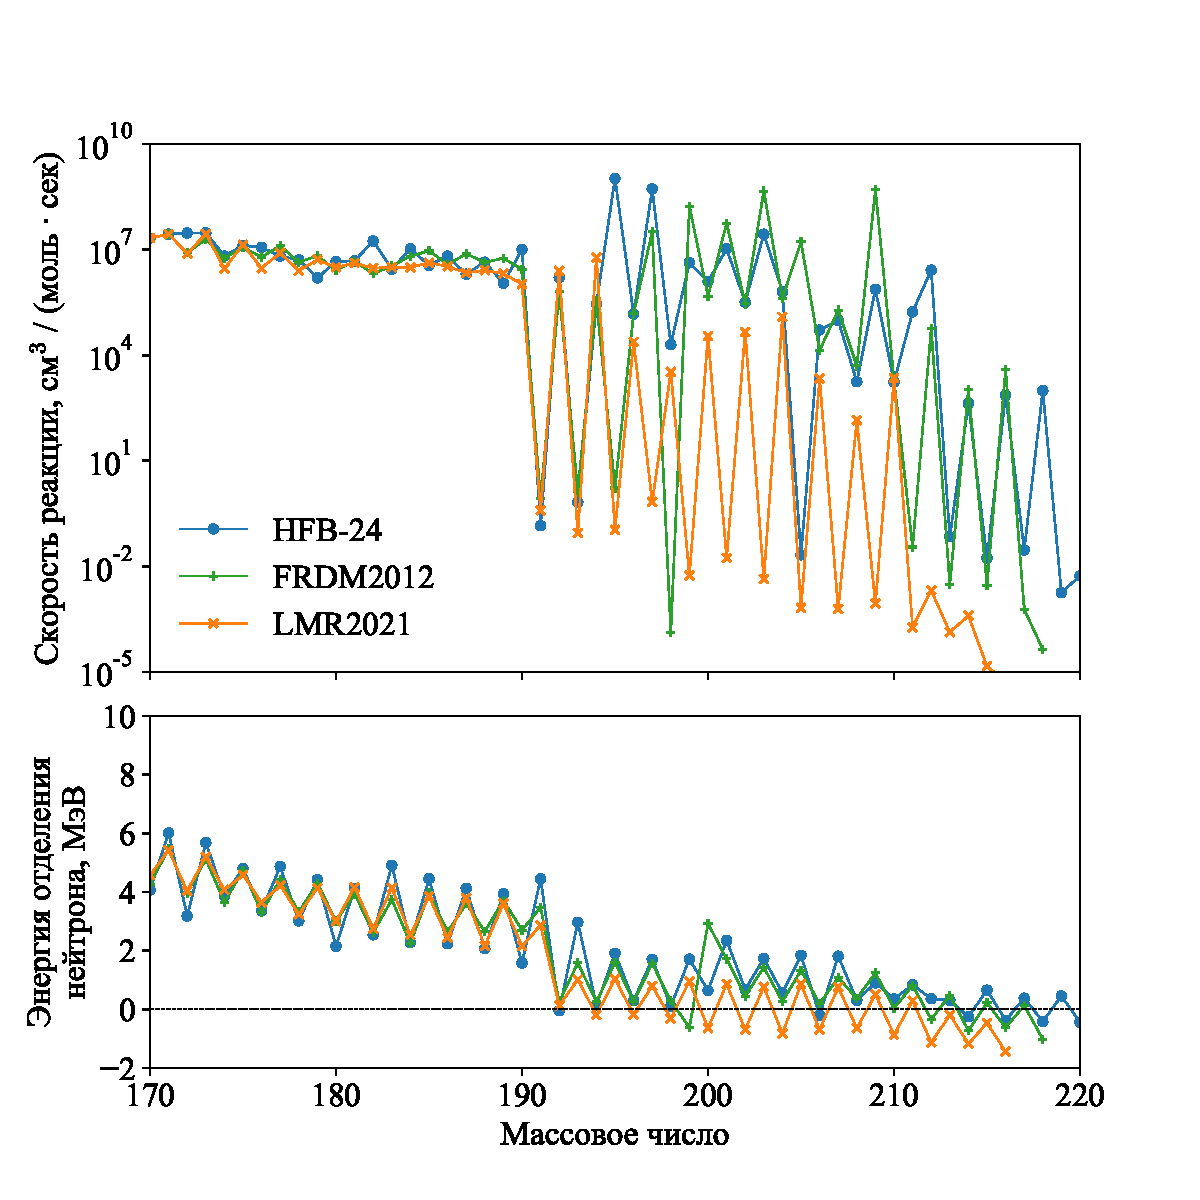
\includegraphics[width=0.6\textwidth]{../pics/rates_vs_A_tb.pdf}
  \caption{Сверху: скорости нейтронных захватов на нейтроноизбыточных изотопах тербия, рассчитанные с помощью различных таблиц ядерных масс при $T = 2$~ГК. Снизу: энергии отделения нейтронов для нейтроноизбыточных изотопов тербия по данным тех же массовых таблиц.}
  \label{fig:rates_vs_A}
\end{figure}

